\chapter{Le Modèle Standard et ses limitations}
\label{sec:ms}

Le Modèle Standard (MS) est une théorie des interactions fondamentales
décrivant la nature avec un niveaux de précision impressionnant.
La structure théorique du modèle est présentée dans la
section~\ref{sec:ms:th}, basée en majeure partie sur les références
\cite{olive_review_2014} et~\cite{thomson_modern_2013}. Quelques grand
problèmes non résolus dans le MS sont exposés dans la
section~\ref{sec:ms:problemes}.

\section{Survol théorique}
\label{sec:ms:th}

Concrètement, le Modèle Standard décrit les particules fondamentales
de la nature ainsi que les forces par lesquelles elles
interagissent. Formellement, les particules
(section~\ref{sec:ms:th:particules}) sont vues comme étant des
excitations localisées de de différents champs dont les interactions
sont décrites par les différents secteurs du Lagrangien du MS
(section~\ref{sec:ms:th:struct}).

\subsection{Les particules du Modèle Standard}
\label{sec:ms:th:particules}

On dénote d'abord deux grands types de particles, défini par la nature
de leur spin. Les particles ayant spin entier sont appelés
\emph{bosons}, tandis que les particules avec spin demi-entier sont
appelés \emph{fermions}. Les fermions sont ensuite séparés en deux
sous-classes, selon leur couleur~\footnote{l'analogue chromodynamique
  de la charge électrique}: les fermions non-colorées sont appelées
\emph{leptons} et ceux ayant une couleur, les \emph{quarks}. Les
propriétés des différentes particules du MS sont résumées dans la
table~\ref{tab:ms_particules}.

Une des caractéristiques frappantes du Modèle Standard est qu'il existe
une \emph{anti-particule} associée à chaque particule. Si la particule
est chargée, son anti-particule a la charge opposée. Le gluon, le
photon et le Z sont leurs propres anti-particules. Il n'est pas encore
clair si les neutrinos sont leurs propres anti-particules.

\begin{table}[h!]
  \centering
  \begin{tabular}{|c|c|c|c|c|c|}
  \hline
  symbole   & nom                 & spin & charge & coloré & Masse \\ \hline
  $\gamma$/$A_\mu$  & photon              & 1    & 0     & non    & 0    \\ \hline
  $g$       & gluon               & 1    & 0     & oui    &  0   \\ \hline
  $Z$       & boson Z             & 1    & 0     & non    & 91.1876 $\pm$ 0.0021 GeV \cite{olive_review_2014} \\ \hline
  $W^-$     & bosons W            & 1    & -1    & non    & 80.385 $\pm$ 0.015 GeV \cite{olive_review_2014} \\ \hline
  $h$       & Higgs               & 0    & 0     & non    & 125.09 $\pm$ 0.21 $\pm$ 0.11 GeV \cite{atlas_collaboration_combined_2015}  \\ \hline
  $e^-$     & électron          & 1/2  & -1    & non    & 0.510998928 $\pm$ 0.000000011 \cite{mohr_codata_2012} \\ \hline
  $\mu^-$   & muon                & 1/2  & -1    & non    & 105.6583715 $\pm$ 0.0000035 MeV \cite{mohr_codata_2012}    \\ \hline
  $\tau^-$  & tau                 & 1/2  & -1    & non    & 1.77686 $\pm$ 0.00012 GeV \cite{olive_review_2014}    \\ \hline
  $\nu_e$   & électron-neutrino & 1/2  & 0     & non    & $\bar{\nu}$: < 2 eV \cite{olive_review_2014} / $\nu$: < 460 eV \cite{yasumi_mass_1994} \\ \hline
  $\nu_\mu$ & muon-neutrino       & 1/2  & 0     & non    & < 0.19 MeV \cite{olive_review_2014}    \\ \hline
  $\nu_\tau$ & tau-neutrino       & 1/2  & 0     & non    &  < 18.2 MeV \cite{al_upper_1998}   \\ \hline
  $d$       & quark down          & 1/2  & -1/3  & oui    & 4.8 + 0.5 - 0.3 MeV \cite{olive_review_2014}     \\ \hline
  $u$       & quark up            & 1/2  & 2/3   & oui    & 2.3 + 0.7 - 0.5 MeV \cite{olive_review_2014}    \\ \hline
  $s$       & quark strange       & 1/2  & -1/3  & oui    & 95 $\pm$ 5 MeV \cite{olive_review_2014}    \\ \hline
  $c$       & quark charm         & 1/2  & 2/3   & oui    & 1.275 $\pm$ 0.025 GeV \cite{olive_review_2014}    \\ \hline
  $b$       & quark bottom        & 1/2  & -1/3  & oui    & 4.18 $\pm$ 0.03 GeV \cite{olive_review_2014}    \\ \hline
  $t$       & quark top           & 1/2  & 2/3   & oui    & 173.21 $\pm$ 0.51 $\pm$ 0.71 GeV \cite{olive_review_2014}    \\ \hline
\end{tabular}
\caption{Les particules du Modèle Standard et leurs propriétés. Chaque particule a une anti-particule associée,
  ayant une charge électrique inverse. Le gluon, le photon, le Z et potentiellement les neutrinos sont leurs
  propres anti-particules. }
\label{tab:ms_particules}
\end{table}

En regardant dans la table~\ref{tab:ms_particules} les masses des
leptons et des quarks, on observe la structure suivante:
\begin{eqnarray}
  m_e < m_\mu < m_\tau \\
  m_d < m_s < m_b \\
  m_u < m_c < m_t 
\end{eqnarray}

On dit donc qu'il y a trois générations de fermions, selon leur
échelle de masse. On associe aussi une génération à chaque neutrino,
selon qu'il sont électroniques (première génération), muoniques
(deuxième génération) ou tauoniques (troisième
génération)~\cite{thomson_modern_2013}.

\subsection{Structure du Modèle Standard}
\label{sec:ms:th:struct}

% Intro
Le Modèle Standard peut être séparé en trois secteurs principaux: le
secteur électrofaible, le secteur Higgs et le secteur chromodynamique.

\subsubsection{Secteur électrofaible}
\label{sec:ms:th:struct:ewk}

% EWK
Les forces faibles et électromagnétiques sont comprises comme étant
deux aspects d'une seule et même force, la force électrofaible, depuis
les travaux de Glashow, Salam et Weinberg dans les années
1960. Le modèle électrofaible prédit
l'existence de quatre champs de jauge: $W^{(1)}_\mu$, $W^{(2)}_\mu$,
$W^{(3)}_\mu$ et $B_\mu$. La théorie prédit deux nombres quantiques
pour chacun de ces bosons: l'isopsin faible, $I^{(3)}_W$, et
l'hypercharge, $Y$. Les bosons W et Z, ainsi que le photon, sont des
combinaisons linéaires de ces bosons:
\begin{eqnarray}
  \label{eq:ewk_mix}
  W^{\pm}_\mu = \frac{1}{\sqrt{2}}(W^{(1)}_\mu \mp W^{(2)}_\mu)  \\
  Z_\mu = -B_\mu\ sin\ \theta_W + W^{(3)}_\mu cos\ \theta_W \\
  A_\mu = B_\mu\ cos\ \theta_W + W^{(3)}_\mu sin\ \theta_W
\end{eqnarray}
L'angle de mélange électrofaible, $\theta_W$, est un paramètre du
modèle. Les nombres quantiques $I^{(3)}_W$ et $Y$ déterminent la
charge électrique à travers la relation
\begin{eqnarray}
  Q = \frac{Y}{2} + I^{(3)}_W
\end{eqnarray}
La constante de couplage électrique, $e$, est reliée à la constante de
couplage faible, $g_W$, à travers l'angle de mélange:
\begin{eqnarray}
  e = g_W\ sin\ \theta_W
\end{eqnarray}

Le boson $Z$ et le photon sont les médiateurs de la force
électrofaible neutre. Les interactions dans ce secteurs conservent la
charge et les nombres leptoniques et baryoniques. Par conséquent, les
couplages possibles sont entre le boson et un paire
fermion-antifermion de même saveur.

Les bosons $W$ sont chargés et conséquemment, la valeur absolue de la
charge des deux particules au sommet doivent être
différente. L'interaction faible chargé est la plus spéciales du MS en
ce sens qu'elle viole la conservation de saveur: les leptons couplent
avec leur neutrinos respectifs et les quarks sont couplés les uns aux
autres, la force des couplages étant donnés par la matrice CKM.

\subsubsection{Secteur Higgs}
% Higgs
Un problème avec la théorie électrofaible est que les bosons sont sans
masses, ce qui est évidemment en désaccord avec les observations
expérimentales (voir table~\ref{tab:ms_particules}). Le champ de Higgs
est donc incorporé au MS pour expliquer le mécanisme par lequel les
bosons électrofaibles acquièrent leurs masses. Une conséquence
expérimentale importante de ce champ est la présence d'un boson
scalaire neutre massif, le Higgs, qui a été confirmée en 2012 par les
expériences ATLAS~\cite{aad_observation_2012} et~CMS~\cite{chatrchyan_observation_2012}.

\subsubsection{Secteur chromodynamique}
% QCD
Le Modèle Standard est complété par le secteur chromodynamique, qui
décrit l'interaction entre particules portant une couleur. Le
médiateur de cette force est le gluon, et il existe seulement des
couplages qqg, ggg et gggg puisque les leptons et les autres bosons ne
sont pas colorés. L'interaction chromodynamique est aussi appelée
force forte.

Une caractéristique importante de cette force est que sa
constante de couplage, $\alpha_s$, décroît lorsque l'échelle d'énergie
augmente: ce phénomène est appelé \emph{liberté asymptotique}. La
figure~\ref{fig:alpha_s} montre un sommaire des principales mesures
d'$\alpha_s$ à diverse échelles d'énergie, confirmant solidement cette
particularité de la théorie.

\begin{figure}
  \centering
  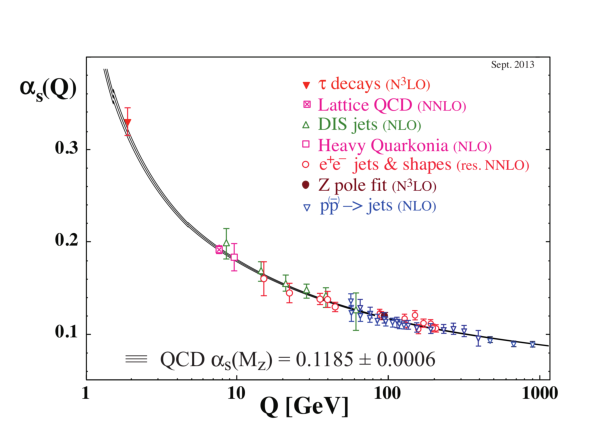
\includegraphics{alpha_s.pdf}
  \caption{Sommaire des principales mesures de la constante de couplage forte, $\alpha_s$, à différentes échelles d'énergies ($Q$). Figure tirée de la réf.~\cite{olive_qcd_2014}.}
\label{fig:alpha_s}
\end{figure}

Une conséquence importe de ce phénomène est que les quarks sont
confinés dans des états liés, puisque la constante de couplage
augmente rapidement alors que l'échelle de distance augmente. Pour
produire des interactions fortes en laboratoire, il faut donc
collisionner des états liés de quarks et gluons, communément appelés
\emph{hadrons}. Or, ceci complique les calculs, puisqu'on ne sait pas
entre quels constituants une interaction donnée a eu lieu. Il faut
donc exprimer les sections efficaces en termes de fonctions de
structures qui paramètrent le contenue en parton~\footnote{parton
  $\equiv$ quark, anti-quark ou gluon} d'un hadron donné. Ces
fonctions ne sont en général pas calculables théoriquement, donc elles
doivent plutôt êtres exprimées en terme des fonctions de densités de
partons (PDF) $f_q(x,Q^2)$ calculées expérimentalement et exprimée en
fonction de la fraction de l'impulsion du hadron porté par le parton
$q$ et l'échelle d'énergie du processus $Q^2$. Une représentation
graphique de la PDF du proton
\texttt{NNPDF2.3}~\cite{ball_parton_2013} est montrée dans la
figure~\ref{fig:pdf}.

\begin{figure}
  \centering
  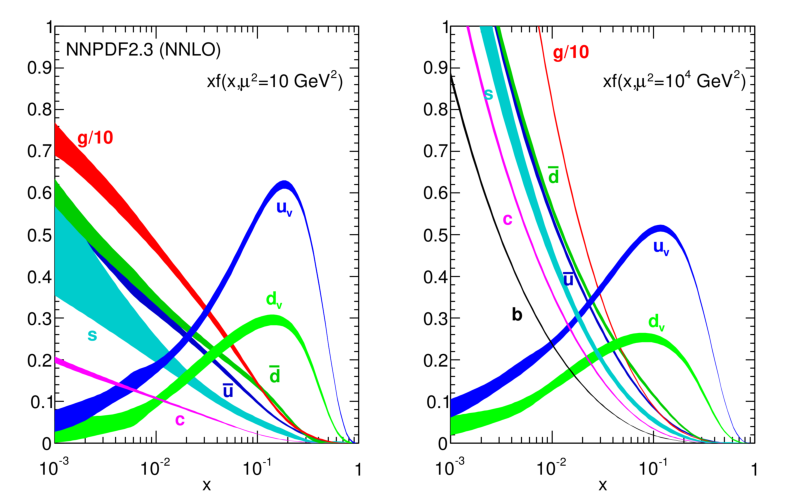
\includegraphics{nnpdf23.pdf}
  \caption{Représentation graphique de la PDF du proton
    \texttt{NNPDF2.3}~\cite{ball_parton_2013}, à deux échelles
    d'énergies ($\mu$) différentes et exprimé en fonction de la
    fraction d'impulsion porté par un parton donné, $x$. Figure tirée de la
    réf. \cite{olive_qcd_2014}.}
  \label{fig:pdf}
\end{figure}

Les interactions peuvent avoir des partons libres dans l'état
final. Or, la liberté asymptotique veut qu'ils soient confinés en
états liés; il y a donc une phase successive d'\emph{hadronisation},
lors de laquelle les quarks irradient des gluons et les gluons se
désintègrent en pairs quarks-antiquarks, de façon à créer une cascade
de hadrons dans l'état final (voir
figure~\ref{fig:hadronisation}). Les hadrons d'une même cascade
tendent à être collimés dans une même direction et forment donc des
dépôts d'énergie dans les calorimètres appelés
\emph{gerbes}~\footnote{Traduction du terme anglais
  «jet»}~\cite{thomson_modern_2013}.

\begin{figure}
  \centering
  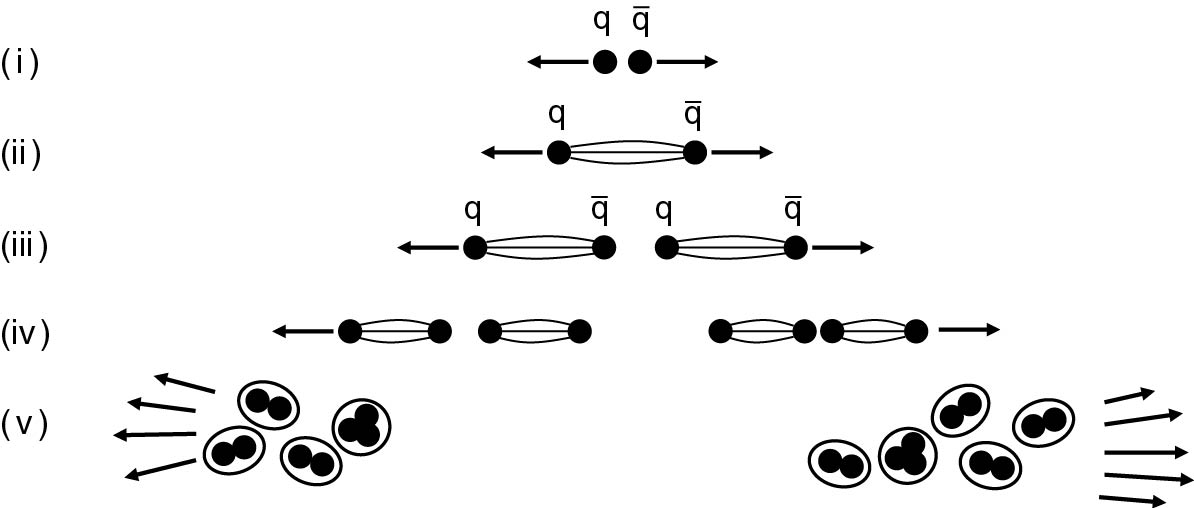
\includegraphics{hadronisation.jpg}
  \caption{Processus d'hadronisation. i) Production d'une pair de
    quarks libres. ii) Échange de gluons entre les quarks. iii,iv) Les
    gluon émetent des paire $q\overline{q}$ à cause de la croissance
    rapide d'$\alpha_s$. v) Formation de hadrons lorsque l'énergie des
    quarks est rendu assez basse. Figure tirée de la
    référence~\cite{thomson_modern_2013}.}
  \label{fig:hadronisation}
\end{figure}

% \section{Validation expérimentale}
% \label{sec:ms:exp}

% \subsection{Mesures du secteur électrofaible}
% \label{sec:ms:exp:ewk}

% \subsection{Mesures du secteur chromodynamique}
% \label{sec:ms:exp:qcd}

% \subsection{Mesures du secteur Higgs}
% \label{sec:ms:exp:Higgs}

\section{Problèmes avec le Modèle Standard}
\label{sec:ms:problemes}

% intro
Malgré le succès phénoménal du Modèle Standard pour décrire la nature
à un niveau fondamental, la théorie contient quelques problèmes
importants qui motivent la recherche de théories sous-jacentes. \\

% Problème de la hiérarchie des masses
Un premier problème, celui de la \emph{hiérarchie des masses}, est
relié à la différence d'énergie importante entre l'échelle faible et
l'échelle de Planck, $M_P$, à laquelle les effets gravitationnels ne
peuvent plus être négligés~\footnote{$M_P = 2.4 \times 10^{18}$~GeV}. Puisque le MS ne décrit pas la gravité,
$M_P$ représente l'énergie à laquelle il faut absolument remplacer la
théorie présente par une plus fondamentale. Il se peut que le MS soit
remplacé à une énergie plus basse que $M_P$; cette échelle est notée $\Lambda_{UV}$.

% correction a la masse
Le problème de la hiérarchie des masses apparaît lorsqu'on considère
les corrections d'ordres supérieures à la masse du Higgs. Le Higgs peut
spontanément émettre une paire fermion-antifermion qui s'annihile
ensuite pour redonner un Higgs~(voir figure~\ref{fig:hloop}). Ce type de diagramme à boucle a pour
effet de modifier la masse du Higgs en ajoutant un terme~\cite{martin_supersymmetry_1997}.:

\begin{eqnarray}
\label{eq:higgs_fermion_corr}
\Delta m_H^2 \propto -\Lambda_{UV}^2
\end{eqnarray}

\begin{figure}
  \centering
  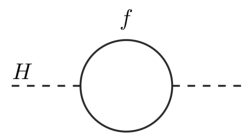
\includegraphics{higgs-loop.pdf}
  \caption{Correction à une boucle de la masse du Higgs par un fermion}
  \label{fig:hloop}
\end{figure}

% Mesure de m_H: fine tuning problem
La masse du Higgs a été mesuré en 2012 par les expériences ATLAS et
CMS et est de
$125.05 \pm 0.24$~GeV~\cite{atlas_collaboration_combined_2015}. Si
$\Lambda_{UV} \approx M_P$, alors la correction du diagramme à boucle
diverge de plusieurs ordres de grandeur par rapport la valeur mesurée
et Il faut alors soit ajuster une constante de proportionnalité à
environ $10^{-22}~\%$~\cite{giudice_naturally_20087} (ce qui est fait
dans le MS) ou remplacer le MS à un échelle $\Lambda_{UV} \ll M_P$ par
une théorie ayant une symétrie protégeant la masse du
Higgs~\cite{martin_supersymmetry_1997}. \\

% Matière sombre
En outre, certaines observations en astrophysique, par exemple dans la
mesure de la courbe de rotation des galaxies, présentent des anomalies
qui impliquent la présence d'amoncellements de particules massives
interagissant seulement par la force faible, appelés
\emph{WIMP}~\footnote{\emph{WIMP} $\equiv$ \emph{Weakly Interacting
    Massive Particle}}. Aucune particules dans le MS n'a les propriété
requises pour expliquer ces anomalies: c'est le problème de la
\emph{Matière Sombre}~\cite{bertone_particle_2005}. \\

% Unification
Un troisième problème théorique avec le MS est celui de
l'\emph{unification des couplages}. Il a été établie dans la
section~\ref{sec:ms:th:struct} que la constante de couplage forte
dépend de l'échelle d'énergie du processus considéré (voir
figure~\ref{fig:alpha_s}). Il en va de même pour les constantes de
couplages faibles et électromagnétiques qui, contrairement à
$\alpha_s$, augmentent en force avec l'échelle d'énergie. Si les
forces fortes, faibles et électriques sont fondamentalement des
manifestations d'une seule et même force dans une théorie
sous-jacente, alors il existe une échelle d'énergie d'unification,
$M_G$, à laquelle une seule constante, $\alpha_G$, définie la magnitude
des interactions. Les constantes de couplages à basse énergie doivent pouvoir
s'exprimer en fonction de $\alpha_G$. Or, une telle unification n'est
pas possible dans le Modèle Standard, et il faut donc considérer des
extensions à la théorie pour la réaliser~\cite{olive_gut_2014,thomson_modern_2013}.


%%% Local Variables:
%%% mode: latex
%%% TeX-master: "memoire"
%%% End:
